\documentclass[../main.tex]{subfiles}

\graphicspath{{../images/}}

\begin{document}
\pagestyle{fancy}
\lhead{Homework 1}
\chead{Junseo Shin}
\rhead{PHYS 421}

\paragraph{1.5}
Proving the ``BAC--CAB'' rule for three-dimensional vectors:
\begin{align*}
    \vb{A} \cp (\vb{B} \cp \vb{C}) &= \vb{A} \cp
    \begin{vmatrix}
        \vu{x} & \vu{y} & \vu{z} \\
        B_x & B_y & B_z \\
        C_x & C_y & C_z
    \end{vmatrix} \\
    &= \begin{vmatrix}
        \vu{x} & \vu{y} & \vu{z} \\
        A_x & A_y & A_z \\
        B_y C_z - B_z C_y & B_z C_x - B_x C_z & B_x C_y - B_y C_x
    \end{vmatrix}
\end{align*}
where the $x$ component is 
\[A_y (B_x C_y - B_y C_x) - A_z (B_z C_x - B_x C_z)\]
From the ``BAC-CAB'' rule,
\begin{align*}
    \vb{B}(\vb{A} \cdot \vb{C}) - \vb{C}(\vb{A} \cdot \vb{B}) &=
        \vb{B} (A_x C_x + A_y C_y + A_z C_z) - \vb{C} (A_x B_x + A_y B_y + A_z B_z)
\end{align*}
where $x$ component simplifes to
\begin{align*}
    B_x (\cancel{A_x C_x} + \textcolor{draculacyan}{A_y C_y} + \textcolor{draculapink}{A_z C_z}) 
        - C_x (\cancel{A_x B_x}+ \textcolor{draculacyan}{A_y B_y} + \textcolor{draculapink}{A_z B_z}) &=
        \textcolor{draculacyan}{A_y (B_x C_y - B_y C_x)} \textcolor{draculapink}{- A_z (B_z C_x - B_x C_z)}
\end{align*}
So,
\[[\vb A \cross (\vb B \cross \vb C)]_x = [\vb B(\vb A \cdot \vb C) - \vb C ( \vb A \cdot \vb B)]_x\]
and similary for the $y$ and $z$ components. Therefore, the ``BAC--CAB'' rule holds true.

\newpage
\paragraph{1.11}
(a) Finding gradient of $f(x, y, z) = x^2 + y^3 + z^4$:
\begin{align*}
    \grad{f} &= \pdv{f}{x} \vu{x} + \pdv{f}{y} \vu{y} + \pdv{f}{z} \vu{z} \\
    &= 2x \vu{x} + 3y^2 \vu{y} + 4z^3 \vu{z}
\end{align*}
(b) Gradient of $f(x, y, z) = x^2y^3z^4$:
\begin{align*}
    \grad{f} = 2xy^3z^4 \vu{x} + 3x^2y^2z^4 \vu{y} + 4x^2y^3z^3 \vu{z}
\end{align*}
(c) Gradient of $f(x, y, z) = e^x \sin(y) \ln(z)$:
\begin{align*}
    \grad{f} = e^x \vu{x} + e^x \cos(y) \ln(z) \vu{y} + \frac{e^x \sin(y)}{z} \vu{z}
\end{align*}

\newpage
\paragraph{1.13}
Given the seperation vector
\begin{align*}
    \boldscriptr = (x - x') \vu{x} + (y - y') \vu{y} + (z - z') \vu{z} \qand 
    \scriptr = \sqrt{(x - x')^2 + (y - y')^2 + (z - z')^2}
\end{align*}
(a) Show that $\grad(\scriptr^2) = 2 \boldscriptr$:
\begin{align*}
    \scriptr^2 = (x - x')^2 + (y - y')^2 + (z - z')^2 
\end{align*}
and each component of the gradient is
\begin{align*}
    \pdv{x}(\scriptr^2) &= 2(x - x') \\
    \pdv{y}(\scriptr^2) &= 2(y - y') \\
    \pdv{z}(\scriptr^2) &= 2(z - z')
\end{align*}
so
\begin{align*}
    \grad(\scriptr^2) &= 2 \boldscriptr
\end{align*}
(b) Show $\grad(1/\scriptr) = -\vu*{\boldscriptr}/\scriptr^2$:
\begin{align*}
    \frac{1}{\scriptr} = [(x - x')^2 + (y - y')^2 + (z - z')^2]^{-1/2} = [(\;)]^{-1/2}
\end{align*}
looking at the $x$ component of the gradient (using chain rule),
\begin{align*}
    \pdv{x}(\frac{1}{\scriptr}) &= -\frac{1}{2} [(\;)]^{-3/2} \cdot 2(x - x') \\
    &= -\frac{(x - x')}{\scriptr^3}
\end{align*}
and similarly for the $y$ and $z$ components:
\begin{align*}
    \grad(\frac{1}{\scriptr}) &= \pdv{x}(\frac{1}{\scriptr}) \vu{x}
        + \pdv{y}(\frac{1}{\scriptr}) \vu{y} + \pdv{z}(\frac{1}{\scriptr}) \vu{z} \\
    &= -\frac{1}{\scriptr^3}
        [(x - x') \vu{x} + (y - y') \vu{y} + (z - z') \vu{z}]
    = -\frac{\boldscriptr}{\scriptr^3}
\end{align*}
Finally, substituting the unit vector $\vu{\boldscriptr} = \boldscriptr/\scriptr$ gives us
\begin{align*}
    \grad(\frac{1}{\scriptr}) = -\frac{\vu*{\boldscriptr}}{\scriptr^2}
\end{align*}
(c) The general formula for $\grad(\scriptr^n)$:
\begin{align*}
    \grad(\scriptr^n) &=
    n \scriptr^{n-1} \cdot \grad{(\scriptr)}
\end{align*}
where
\begin{align*}
    \grad{(\scriptr)} &= \pdv{x}(\scriptr) \vu{x} + \pdv{y}(\scriptr) \vu{y} + \pdv{z}(\scriptr) \vu{z} \\
    &= \frac{1}{2} [(\;)]^{-1/2} \cdot 2(x - x') \vu{x} + \dots \qqtext{[similar to part (b)]} \\
    &= \frac{\boldscriptr}{\scriptr} = \vu{\boldscriptr}
\end{align*}
So the general formula is
\begin{align*}
    \grad(\scriptr^n) = n \scriptr^{n-1} \vu{\boldscriptr}
\end{align*}

\newpage
\paragraph{1.15}
(a) Calculating divergence of $\vb v_a = x^2\vu{x} + 3xz^2\vu{y} - 2xz\vu{z}$:
\begin{align*}
    \div{\vb v_a} &= \pdv{v_{ax}}{x} + \pdv{v_{ay}}{y} + \pdv{v_{az}}{z} \\
    &= 2x + 0 - 2x = 0
\end{align*}

(b) $\vb v_b = xy\vu{x} + 2yz\vu{y} + 3zx\vu{z}$:
\begin{align*}
    \div{\vb v_b} &= y + 2z + 3x
\end{align*}

(c) $\vb v_c = y^2\vu{x} + (2xy + z^2)\vu{y} + 2yz\vu{z}$:
\begin{align*}
    \div{\vb v_c} &= 0 + 2x + 2y = 2(x + y)
\end{align*}

\newpage
\paragraph*{1.16}
\begin{figure*}[ht]
    \centering
    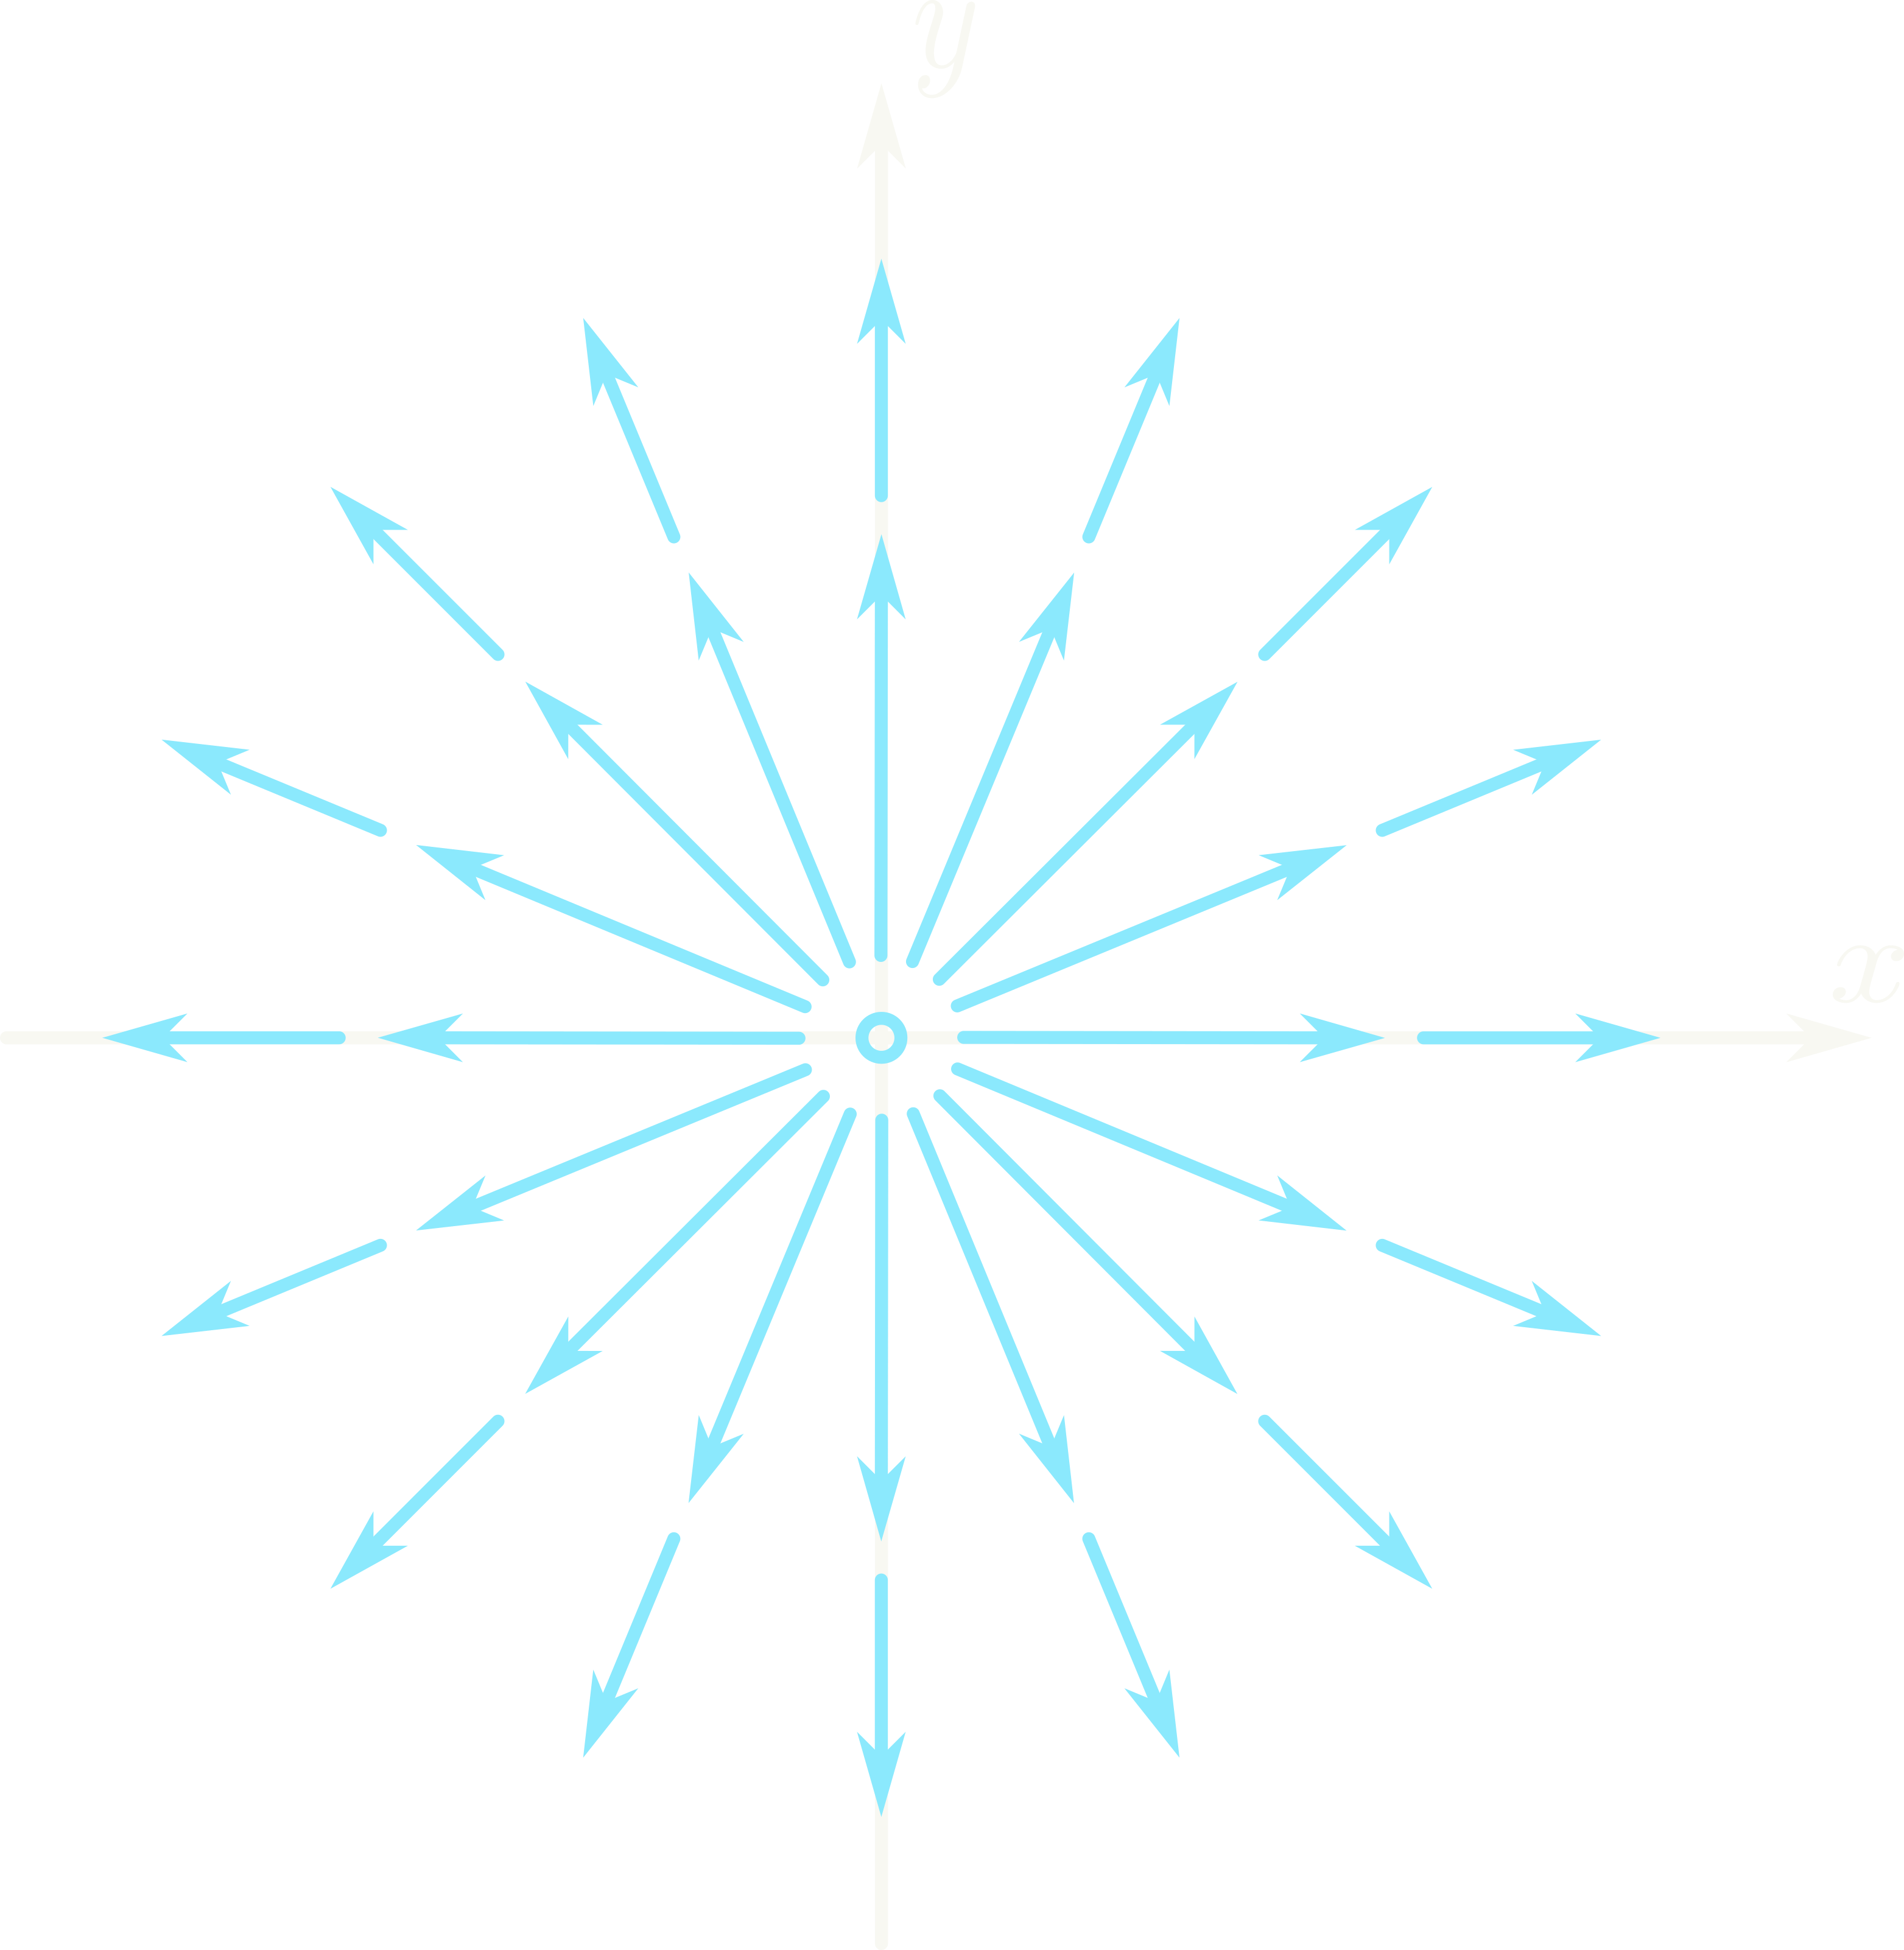
\includegraphics[width=0.4\textwidth]{fighw1.png}
    \renewcommand{\thefigure}{1.16}
    \caption{The vector field $\vb v = \frac{\vu r}{r^2}$}
    \label{fig:1.16}
\end{figure*}
Given
\begin{align*}
    r = \sqrt{x^2 + y^2 + z^2} \qand
    \vu{r} = \frac{\vb{r}}{r} = \frac{x\vu{x} + y\vu{y} + z\vu{z}}{\sqrt{x^2 + y^2 + z^2}}
\end{align*}
where $\vb{r} = x\vu{x} + y\vu{y} + z\vu{z}$ is the position vector. The vector functions is
\begin{align*}
    v = \frac{\vu{r}}{r^2} = \frac{\vb{r}}{r^3}
\end{align*}
where the components are
\begin{align*}
    v_x = \frac{x}{r^3}, \quad v_y = \frac{y}{r^3}, \qand v_z = \frac{z}{r^3}
\end{align*}
Looking at the $x$ component of the divergence,
\begin{align*}
    [\div{\vb{v}}]_x &= \pdv{v_x}{x} \\
    &= \pdv{x}(\frac{x}{r^3}) \\
    &= \pdv{x}(\frac{x}{(x^2 + y^2 + z^2)^{3/2}}) \qq{using chain rule...}\\
    &= \frac{1}{(x^2 + y^2 + z^2)^{3/2}} - \frac{3x^2}{(x^2 + y^2 + z^2)^{5/2}} \\
    &= \frac{1}{r^3} - \frac{3x^2}{r^5}
\end{align*}
therefore, the divergence of $\vb{v}$ is
\begin{align*}
    \div{\vb{v}} &= \quantity(\frac{1}{r^3} - \frac{3x^2}{r^5})
        + \quantity(\frac{1}{r^3} - \frac{3y^2}{r^5})
        + \quantity(\frac{1}{r^3} - \frac{3z^2}{r^5}) \\
    &= \frac{3}{r^3} - 3\frac{x^2 + y^2 + z^2}{r^5} \\
    &= \frac{3}{r^3} - 3\frac{r^2}{r^5} = 0
\end{align*}
The divergence is zero everywhere except at the origin where $r = 0$ because division by $r^3$ tells us that the divergence is infinite at the origin.

\newpage
\paragraph*{1.18}
Curl of vector functions from Problem 1.15:
(a) $\vb{v}_a = x^2\vu{x} + 3xz^2\vu{y} - 2xz\vu{z}$:
\begin{align*}
    \curl{\vb{v}_a} &= \mqty|
        \vu{x} & \vu{y} & \vu{z} \\
        \pdv{x} & \pdv{y} & \pdv{z} \\
        x^2 & 3xz^2 & -2xz
    | \\
    &= \vu{x} (0 - 6xz) - \vu{y} (-2z - 0) + \vu{z} (3z^2 - 0) \\
    &= -6xz\vu{x} + 2z\vu{y} + 3z^2\vu{z}
\end{align*}

(b) $\vb{v}_b = xy\vu{x} + 2yz\vu{y} + 3zx\vu{z}$:
\begin{align*}
    \curl{\vb{v}_b} &= \begin{vmatrix}
        \vu{x} & \vu{y} & \vu{z} \\
        \pdv{x} & \pdv{y} & \pdv{z} \\
        xy & 2yz & 3zx
    \end{vmatrix} \\
    &= \vu{x} (0 - 2y) - \vu{y} (3z - 0) + \vu{z} (0 - x) \\
    &= -2y\vu{x} - 3z\vu{y} - x\vu{z}
\end{align*}

(c) $\vb{v}_c = y^2\vu{x} + (2xy + z^2)\vu{y} + 2yz\vu{z}$:
\begin{align*}
    \curl{\vb{v}_c} &= \begin{vmatrix}
        \vu{x} & \vu{y} & \vu{z} \\
        \pdv{x} & \pdv{y} & \pdv{z} \\
        y^2 & 2xy + z^2 & 2yz
    \end{vmatrix} \\
    &= \vu{x} (2z - 2z) - \vu{y} (0 - 0) + \vu{z} (2y - 2y) \\
    &= 0
\end{align*}

\newpage
\paragraph{1.32}
Given $T = x^2 + 4xy + 2yz^3$,
\begin{align*}
    \pdv{T}{x} = 2x + 4y  ,\quad     \pdv{T}{y} = 4x + 2z^3  ,\qand   \pdv{T}{z} = 6yz^2
\end{align*}
therefore
\begin{align*}
    \grad{T} = \vu{x}(2x + 4y) + \vu{y}(4x + 2z^3) + \vu{z}(6yz^2)
\end{align*}
Checking the fundamental theorem for gradients using the points $a = (0,0,0) \to b = (1,1,1)$:
\begin{align*}
    \int_a^b \grad{T} \vdot \dd{\vb{l}} = T(b) - T(a) = 1^2 + 4(1)(1) + 2(1)(1)^3 - 0 = 7
\end{align*}
For the three paths:
\begin{itemize}
    \item[(a)] $a \to (1,0,0) \to (1,1,0) \to b$;
    \begin{enumerate}
        \item[(i)] $a \to (1,0,0)$:
        \begin{align*}
                x: 0 \to 1; \quad y = z = \dd{y} = \dd{z} = 0; \quad \dd{\vb{l}} = \dd{x} \vu{x};
                \quad \grad{T} \vdot \dd{\vb{l}} = 2x \dd{x}
        \end{align*}
        and
        \begin{align*}
            \int_a^c \grad{T} \vdot \dd{\vb{l}} = \int_0^1 2x \dd{x} = 1
        \end{align*}
        \item[(ii)] $(1,0,0) \to (1,1,0)$:
        \begin{align*}
            y: 0 \to 1; \quad x = 1, \quad z = \dd{x} = \dd{z} = 0; \quad \dd{\vb{l}} = \dd{y} \vu{y};
                \quad \grad{T} \vdot \dd{\vb{l}} = 4 \dd{y}
        \end{align*}
        and
        \begin{align*}
            \int_c^d \grad{T} \vdot \dd{\vb{l}} = \int_0^1 4 \dd{y} = 4
        \end{align*}
        \item[(iii)] $(1,1,0) \to b$:
        \begin{align*}
            z: 0 \to 1; \quad x = y = 1, \quad \dd{x} = \dd{y} = 0; \quad \dd{\vb{l}} = \dd{z} \vu{z};
                \quad \grad{T} \vdot \dd{\vb{l}} = 6z^2 \dd{z}
        \end{align*}
        and
        \begin{align*}
            \int_d^b \grad{T} \vdot \dd{\vb{l}} = \int_0^1 6z^2 \dd{z} = 2
        \end{align*}
        therefore
        \begin{align*}
            \int_a^b \grad{T} \vdot \dd{\vb{l}} = 1 + 4 + 2 = 7
        \end{align*}
    \end{enumerate}
    \item[(b)] $a \to (0,0,1) \to (0,1,1) \to b$;
    \begin{enumerate}
        \item [(i)] $a \to (0,0,1)$:
        \begin{align*}
            z: 0 \to 1;\quad x = y = \dd{x} = \dd{y} = 0; \quad \dd{\vb{l}} = \dd{z} \vu{z};
                \quad \grad{T} \vdot \dd{\vb{l}} = 0
        \end{align*}
        and
        \begin{align*}
            \int_a^c \grad{T} \vdot \dd{\vb{l}} = \int_0^1 0 = 0
        \end{align*}
        \item [(ii)] $(0,0,1) \to (0,1,1)$:
        \begin{align*}
            z = 1, \quad x = \dd{x} = \dd{z} = 0; \quad \dd{\vb{l}} = \dd{y} \vu{y};
                \quad \grad{T} \vdot \dd{\vb{l}} = 2 \dd{y}
        \end{align*}
        and
        \begin{align*}
            \int_c^d \grad{T} \vdot \dd{\vb{l}} = \int_0^1 2 \dd{y} = 2
        \end{align*}
        \item [(iii)] $(0,1,1) \to b$:
        \begin{align*}
            z: 0 \to 1 ;\quad y = z = 1, \quad \dd{y} = \dd{z} = 0; \quad \dd{\vb{l}} = \dd{x} \vu{x};
                \quad \grad{T} \vdot \dd{\vb{l}} = (2x+4) \dd{x}
        \end{align*}
        and
        \begin{align*}
            \int_d^b \grad{T} \vdot \dd{\vb{l}} = \int_0^1 (2x+4) \dd{x} = 5
        \end{align*}
        therefore
        \begin{align*}
            \int_a^b \grad{T} \vdot \dd{\vb{l}} = 0 + 2 + 5 = 7
        \end{align*}
    \end{enumerate}
    \item[(c)] the parabolic path $z = x^2$; $y = x$:
    \begin{align*}
        \dd{x} = \dd{y}, \qand \dd{z} = 2x \dd{x}; \quad
        \dd{\vb{l}} = \dd{x} \vu{x} + \dd{x} \vu{y} + 2x\dd{x} \vu{z}
    \end{align*}
    and
    \begin{align*}
        \grad{T} \vdot \dd{\vb{l}} &= (2x+4y) \dd{x} + (4x+2z^3) \dd{x} + (6yz^2) 2x\dd{x} \\
        &= 6x \dd{x} + (4x + 2x^6) \dd{x} + (12x^6) \dd{x} \\
        &= 10x \dd{x} + 14x^6 \dd{x}
    \end{align*}
    therefore
    \begin{align*}
        \int_a^b \grad{T} \vdot \dd{\vb{l}} &= \int_0^1 (10x + 14x^6) \dd{x} \\
        &= \eval{5x^2 + 2x^7}_0^1 = 7
    \end{align*}
\end{itemize}

\newpage
\paragraph{1.33}
Testing the divergence theorem: For the function
\begin{align*}
    \vb{v} = (xy) \vu{x} + (2yz) \vu{y} + (3zx)\vu{z}
\end{align*}
the divergence is
\begin{align*}
    \div{\vb{v}} = y + 2z + 3x
\end{align*}
so the volume integral is
\begin{align*}
    \int_V \div{\vb{v}} \dd{\tau} &= \int_0^2 \int_0^2 \int_0^2(y + 2z + 3x) \dd{x}\dd{y}\dd{z} \\
    &= \int_0^2 \int_0^2 (2y + 4z + 6) \dd{y}\dd{z} \\
    &= \int_0^2 (4 + 8z + 12) \dd{z} \\
    &= 8 + 16 + 24 \\
    \int_V \div{\vb v} \dd{\tau} &= 48
\end{align*}
The surface integral is evaluated over the six faces of the cube:
\begin{enumerate}
    \item [(i)] $x = 2$, $\dd{\vb{A}} = \dd{y}\dd{z} \vu{x}$, $\vb{v} \vdot \dd{\vb{A}} = 2y \dd{y}\dd{z}$;
    \begin{align*}
        \int \vb{v} \vdot \dd{\vb{A}} &= \int_0^2 \int_0^2 2y \dd{y}\dd{z} = 8
    \end{align*}
    \item [(ii)] $x = 0$, $\dd{\vb{A}} = -\dd{y}\dd{z} \vu{x}$, $\vb{v} \vdot \dd{\vb{A}} = 0$;
    \begin{align*}
        \int \vb{v} \vdot \dd{\vb{A}} &= \int_0^2 \int_0^2 0 \dd{y}\dd{z} = 0
    \end{align*}
    \item [(iii)] $y = 2$, $\dd{\vb{A}} = \dd{x}\dd{z} \vu{y}$, $\vb{v} \vdot \dd{\vb{A}} = 4z \dd{x}\dd{z}$;
    \begin{align*}
        \int \vb{v} \vdot \dd{\vb{A}} &= \int_0^2 \int_0^2 4z \dd{x}\dd{z} = 16
    \end{align*}
    \item [(iv)] $y = 0$;
    \begin{align*}
        \int \vb{v} \vdot \dd{\vb{A}} &= 0
    \end{align*}
    \item [(v)] $z = 2$, $\dd{\vb{A}} = \dd{x}\dd{y} \vu{z}$, $\vb{v} \vdot \dd{\vb{A}} = 6x \dd{x}\dd{y}$;
    \begin{align*}
        \int \vb{v} \vdot \dd{\vb{A}} &= \int_0^2 \int_0^2 6x \dd{x}\dd{y} = 24
    \end{align*}
    \item [(vi)] $z = 0$;
    \begin{align*}
        \int \vb{v} \vdot \dd{\vb{A}} &= 0
    \end{align*}
\end{enumerate}
So the total flux is
\begin{align*}
    \oint_S \vb{v} \vdot \dd{\vb{A}} &= 8 + 0 + 16 + 0 + 24 + 0 = 48
\end{align*}
therefore, the divergence theorem is verified.
\begin{align*}
    \int_V (\div{\vb{v}}) \dd{\tau} &= \oint_S \vb{v} \vdot \dd{\vb{A}}
\end{align*}

\newpage
\paragraph{1.34}
Testing Stokes' theorem for the function
\begin{align*}
    \vb{v} = (xy) \vu{x} + (2yz) \vu{y} + (3zx)\vu{z}
\end{align*}
using the triangular shaded area bounded by the vertices
$O = (0,0,0)$, $A = (0,2,0)$, and $B = (0,0,2)$:
\begin{align*}
    \curl{\vb{v}} &= (0 - 2y) \vu{x} - (3z - 0) \vu{y} + (0 - x) \vu{z}
                                                        \qand \dd{\vb{A}} = \dd{z}\dd{y} \vu{x} \\
                  &= -2y \vu{x} - 3z \vu{y} - x \vu{z}
\end{align*}
$x=0$ on this surface, and the limits of integration are $y: 0 \to 2$ and $z = 0 \to z = 2 - y$:
\begin{align*}
    (\curl{\vb{v}}) \vdot \dd{\vb{A}} &= -2y \dd{z}\dd{y}
\end{align*}
Thus, the flux of the curl through the surface is
\begin{align*}
    \int_S (\curl{\vb{v}}) \vdot \dd{\vb{A}} &= \int_0^2 \int_0^{2-y} -2y \dd{z}\dd{y} \\
    &= \int_0^2 -2y(2-y) \dd{y} \\
    &= -2y^2 + \frac{2}{3} y^3 \eval_0^2 = -8/3
\end{align*}
The line integral is evaluated over the three sides of the triangle:
\begin{enumerate}
    \item [(i)] On the path $OA$: \\
    $x = z = 0$; $\dd{\vb{l}} = \dd{y} \vu{y}$; $\vb{v} \vdot \dd{\vb{l}} = 2yz \dd{y} = 0$;
    \begin{align*}
        \int_{OA} \vb{v} \vdot \dd{\vb{l}} &= 0
    \end{align*}
    \item [(ii)] On the path $AB$: \\
    $x = 0$, $y = 2 - z$; $\dd{y} = -\dd{z}$; $\dd{\vb{l}} = -\dd{z}(\vu{y} - \vu{z})$;
    $\vb{v} \vdot \dd{\vb{l}} = -2yz \dd{z} = -2(2 - z)z \dd{z} = (2z^2 - 4z) \dd{z}$;
    \begin{align*}
        \int_{AB} \vb{v} \vdot \dd{\vb{l}} &= \int_0^2 (2z^2 - 4z) \dd{z} = -8/3
    \end{align*}
    \item [(iii)] On the path $BO$: \\
    $x = y = 0$; $\dd{\vb{l}} = \dd{z} \vu{z}$; $\vb{v} \vdot \dd{\vb{l}} = 0$;
    \begin{align*}
        \int_{BO} \vb{v} \vdot \dd{\vb{l}} &= 0
    \end{align*}
\end{enumerate}
So, the circulation of $\vb{v}$ around the triangle is
\begin{align*}
    \oint \vb{v} \vdot \dd{\vb{l}} &= 0 + -8/3 + 0 = -8/3
\end{align*}
thus,
\begin{align*}
    \int_S (\curl{\vb{v}}) \vdot \dd{\vb{A}} &= \oint \vb{v} \vdot \dd{\vb{l}}
\end{align*}

\end{document}